% Standalone source for the hcinfer user-facing workflow diagram.
% Ported verbatim from hcinfer-stat/hcinfer-stat_v1b.tex (preamble lines
% 39 to 162 and the tikzpicture at lines 327 to 355). Compile with
% latexmk -pdf then convert to PNG with pdftools::pdf_convert at 300 DPI.
\documentclass[border=5pt]{standalone}
\usepackage{tikz}
\usetikzlibrary{arrows.meta,backgrounds,calc,fit,positioning,shapes.geometric}

\definecolor{codebg}{HTML}{F7F8FA}
\definecolor{codeframe}{HTML}{E1E5EA}
\definecolor{codetext}{HTML}{243746}
\definecolor{codemuted}{HTML}{7A8896}
\definecolor{codestring}{HTML}{2C5F8A}
\definecolor{hcink}{HTML}{243746}
\definecolor{hcpage}{HTML}{FFFFFF}
\definecolor{hcapi}{HTML}{2C5F8A}
\definecolor{hcapifill}{HTML}{F2F6FA}
\definecolor{hccorecol}{HTML}{3D6B5D}
\definecolor{hccorefill}{HTML}{F3F7F5}
\definecolor{hcobject}{HTML}{6A5D84}
\definecolor{hcobjectfill}{HTML}{F6F4F8}
\definecolor{hcsupport}{HTML}{8A8F94}
\definecolor{hcsupportfill}{HTML}{F7F8FA}
\definecolor{hcline}{HTML}{6D7680}
\definecolor{hcfaint}{HTML}{A9B2BA}

\tikzset{
  hcblock/.style={
    draw=hcink,
    rounded corners=3pt,
    line width=0.55pt,
    fill=hcpage,
    align=center,
    minimum height=7mm,
    inner xsep=6pt,
    inner ysep=3pt,
    font=\normalsize\bfseries\ttfamily,
    text=hcink
  },
  hcentry/.style={
    hcblock,
    fill=hcink,
    text=hcpage,
    minimum width=23mm
  },
  hccore/.style={
    hcblock,
    draw=hcapi,
    fill=hcapifill,
    text=hcapi,
    line width=0.75pt,
    minimum width=30mm
  },
  hcleaf/.style={
    hcblock,
    draw=hcapi,
    text=hcapi,
    minimum width=25mm,
    font=\scriptsize\bfseries\ttfamily
  },
  hcpanel/.style={
    draw=hcsupport,
    fill=hcsupportfill,
    rounded corners=8pt,
    line width=0.6pt,
    inner sep=7pt
  },
  hccard/.style={
    draw=hcsupport,
    fill=hcsupportfill,
    rounded corners=8pt,
    line width=0.6pt,
    text=hcink,
    align=left,
    text width=56mm,
    inner xsep=8pt,
    inner ysep=7pt,
    font=\small\sffamily
  },
  hcedge/.style={
    -{Stealth[length=2.2mm,width=1.6mm]},
    line width=0.55pt,
    color=hcline,
    rounded corners=6pt
  },
  hcinternaledge/.style={
    -{Stealth[length=1.9mm,width=1.3mm]},
    line width=0.42pt,
    color=hcfaint,
    densely dashed,
    rounded corners=5pt
  },
  hcsplit/.style={
    line width=0.35pt,
    color=hcfaint
  },
  hclabel/.style={
    font=\scriptsize\sffamily,
    text=hcline,
    align=center
  },
  hcgroup/.style={
    font=\scriptsize\sffamily\bfseries,
    text=hcink
  }
}

\begin{document}
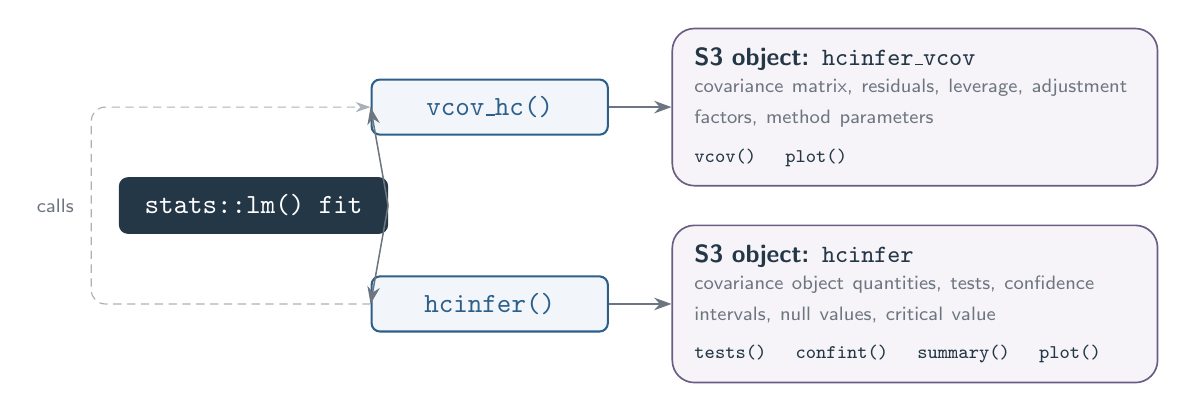
\begin{tikzpicture}[x=1cm,y=1cm]
  \node[hcentry, minimum width=34mm] (fit) at (0,0) {stats::lm() fit};

  \node[hccore] (vcovhc) at (3.0,1.25) {vcov\_hc()};

  \node[hccore] (hcinferfun) at (3.0,-1.25) {hcinfer()};

  \node[hccard, draw=hcobject, fill=hcobjectfill] (covcard) at (8.4,1.25) {%
    \textbf{S3 object: \texttt{hcinfer\_vcov}}\\[-1pt]
    {\scriptsize\color{hcline} covariance matrix, residuals, leverage, adjustment factors, method parameters}\\[3pt]
    {\scriptsize\bfseries\ttfamily vcov() \quad plot()}
  };

  \node[hccard, draw=hcobject, fill=hcobjectfill] (infercard) at (8.4,-1.25) {%
    \textbf{S3 object: \texttt{hcinfer}}\\[-1pt]
    {\scriptsize\color{hcline} covariance object quantities, tests, confidence intervals, null values, critical value}\\[3pt]
    {\scriptsize\bfseries\ttfamily tests() \quad confint() \quad summary() \quad plot()}
  };

  \draw[hcedge] (fit.east) -- (vcovhc.west);
  \draw[hcedge] (fit.east) -- (hcinferfun.west);
  \coordinate (calllower) at ($(fit.west)+(-0.35,-1.25)$);
  \coordinate (callupper) at ($(fit.west)+(-0.35,1.25)$);
  \draw[hcinternaledge] (hcinferfun.west) -- (calllower)
    -- node[hclabel, left=1mm] {calls} (callupper)
    -- (vcovhc.west);
  \draw[hcedge] (vcovhc.east) -- (covcard.west);
  \draw[hcedge] (hcinferfun.east) -- (infercard.west);
\end{tikzpicture}
\end{document}
